\documentclass[9pt,twocolumn,twoside]{idsi}
\setboolean{minireview}{false}
\usepackage{tikz}
\usetikzlibrary{automata, positioning}
\usepackage{listings}
\usepackage{comment}
\usetikzlibrary{trees}
\title{Creating Generative Models by Implementing Markov Chain Monte Carlo Methods Using Spark GraphFrame}


\author[1]{Teja Ambati}
\author[1]{Tyson Trauger}
\author[1, 2]{Professor Robert J. Brunner}

\affil[1]{University of Illinois at Urbana-Champaign}
\affil[2]{Laboratory for Computation, Data, and Machine Learning}


\begin{abstract}
GraphFrame in Spark has many practical applications, including representing Markov chains in large clusters. These Markov chains can be useful in creating generative models. This paper will detail how Spark combined with GraphFrames can be used to represent large Markov chains of words to generate random texts in the style of a specific author.
\end{abstract}

\setboolean{displaycopyright}{false}

\begin{document}
\coverpage{Creating Generative Models by Implementing Markov Chain Monte Carlo Methods Using Spark GraphFrame}{Teja Ambati\\Tyson Trauger\\Professor Brunner}
\maketitle
\section{Introduction}

Model generation requires output to closely match the behavior of extensive input data. This is often done by analyzing the probability of one state going to another state i.e. in terms of sentences, the probability that the word "man" will follow "the". Given a random current state, Markov chains return a possible future state based on probabilities calculated with previously analyzed data. Markov chains could be represented by adjacency lists, but when data becomes sufficiently large, operations on the adjacency list can be very time consuming. In order to sidestep these limitations, Markov chains can be implemented in Apache Spark using GraphFrame. Users with exorbitant amounts of probability based data can analyze the data using distributed computing, which enables them to analyze data much more efficiently than they could with a single computer. In this paper, we explore using Markov chain Monte Carlo methods to create sentences that are in the style of a given author. 

Books, specifically books written by Charles Dickens, were used to represent probability data, where each word has a list of weighted probable future words. By analyzing enough of this data, the Markov chain created a model which could generate text that closely matches the style of Charles Dickens. These concepts could be extended to generate models for any kind of input data, not just sentences in the style of an author. 


\section{Assumptions}
It is assumed that Spark is setup with GraphFrame and one has basic knowledge of how to use Spark and Spark DataFrames.

\section{Graphs}\label{sec:graphs}
Graphs are a way to understand data and relations between them. Every graph is composed of vertices and edges, where vertices are points and edges represent the connection between points. There are two main types of graphs: directed and undirected. In a directed graph each edge is directed from one vertex to another. This means that edges are not bidirectional. For example, if a graph only contains one edge that connects vertex A and vertex B, it is impossible to travel from vertex B to A. \linebreak
 

\begin{figure}[h!]

        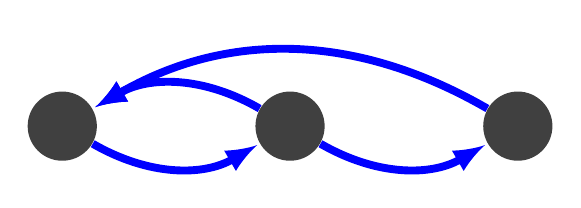
\begin{tikzpicture}[font=\sffamily]
        \node[state,
              text=white,
              draw=none,
              fill=gray!50!black] (s) {};
        \node[state,
              right=2cm of s,
              text=white!30!white, 
              draw=none, 
              fill=gray!50!black] (r) {};
		\node[state,
              right=2cm of r,
              text=white!30!white, 
              draw=none, 
              fill=gray!50!black] (t) {};
        \draw[every loop,
              auto=right,
              line width=1mm,
              >=latex,
              draw=blue,
              fill=blue]
            (s) edge[bend right, auto=left]  node {} (r)
            (r) edge[bend right, auto=right] node {} (s)
            (r) edge[bend right, auto=left] node {} (t)
            (t) edge[bend right, auto=right] node {} (s);
       \end{tikzpicture}
       \caption{A directed graph}\label{fig:directed-graph}
\end{figure}
When talking about graphs in this paper, it is assumed that they are directed unless otherwise noted.

\section{Markov Chains}\label{sec:markov-chains}
Markov chains are a way of simulating random events that are conditional on a current state. Markov chains also have an important property that the history of states, leading up to the current state, have no influence on the future - a property known as memorylessness.\cite{Laurie:1} Markov chains can be represented by a graph: the states are represented as vertices and the edges represent the probability that the next state will be the destination vertex of the step.
\begin{figure}[h!]
    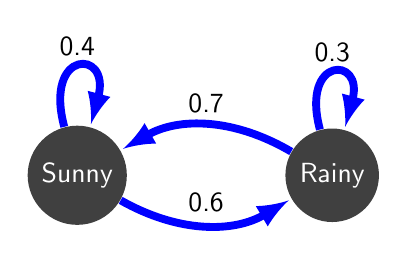
\begin{tikzpicture}[font=\sffamily]
 
    \node[state,
          text=white,
          draw=none,
          fill=gray!50!black] (s) {Sunny};
    \node[state,
          right=2cm of s,
          text=white!30!white, 
          draw=none, 
          fill=gray!50!black] (r) {Rainy};
 
    \draw[every loop,
          auto=right,
          line width=1mm,
          >=latex,
          draw=blue,
          fill=blue]
        (s) edge[bend right, auto=left]  node {0.6} (r)
        (r) edge[bend right, auto=right] node {0.7} (s)
        (s) edge[loop above]             node {0.4} (s)
        (r) edge[loop above]             node {0.3} (r);
   \end{tikzpicture}
   \caption{A graph that represents a Markov chain}\label{fig:markov-chain-graph}
\end{figure}
   \linebreak
   However, a more common way to represent Markov chains is by using a matrix like the figure below.
   
    \begin{equation}
		\left(\begin{array}{cc} .4 & .6\\ .7 & .3\end{array}\right)
	\end{equation}
    Using this notation, Markov chains are represented as transition matrices. Each entry \textit{i,j}, where $i$ is the row and $j$ is the column, represents the probability that the current state \textit{i} will transition to the future state \textit{j}. The columns represent the vertices of the graph and the entries of each column represent the weighted edges connecting the vertices.  
The values in the matrix represent the probability that a given current state will transition to a given future state. Thus, all of the values in a given row must add up to 1. 
    The above matrix represents the same Markov chain as outlined before. The first row represents going from the "Sunny" state to another state and the second row represents going from the "Rainy" state to another state. The first column, on the other hand, represents going from another state to the "Sunny" state and the second column is the same for the "Rainy" state. For example, using the representation above, there is a 60\% chance that "Sunny" will transition to "Rainy".  

\section{Generative Models}
A generative model specifies a joint probability distribution that can be used for sampling from data. The model takes in a parameter, and then evaluates all possible outcomes given that parameter and selects the most likely one based on all of the conditional outcome's possibilities. \cite{Ng:5}

In this paper, a generative model is created using a Markov chain where a vertex is the input parameter and all of the edges represent the probabilities that the destination vertex will be selected. Specifically, this paper deals with words as vertices and the edges as the probability that a word is followed by the destination word. 

\section{Markov Chain Monte Carlo Method}
Markov chain Monte Carlo (MCMC) methods are a set of algorithms that use Markov chains to create a generative model from data. While many different types exist, the one implemented here is of the subset Random Walk Markov Chain.
The algorithm first takes in the data and then generates the samples using a random walk from a given node. 


\section{Spark GraphFrame}
Spark includes a package named GraphFrame that is useful when dealing with problems that can be represented in a graph format. Once you import GraphFrame, a GraphFrame can be initialized by passing it two Spark dataframes, one for the vertices (with ["id",$"value1"$,$"value2"$,...,$"valueN"$] schema) and one for the edges (with ["src","dst",$"edge name"$] schema). Note that GraphFrame requires the first value in the vertices schema to be called "id" and that the first two values in the edges schema to be called "src"(for source vertex) and "dst"(for destination vertex). Example creation of a GraphFrame is shown below:

\begin{lstlisting}[language=python]
from graphframes import *
vertices = sqlContext.createDataFrame([
("A","A_VALUE"),
("B","B_VALUE"),
("C","C_VALUE")
], ["id","EXAMPLE_NAME"])

edges = sqlContext.createDataFrame([
("A","B","follows"),
("B","C","follows"),
("C","B","dislikes")
],["src","dst","EXAMPLE_EDGES"])
	
graphFrame = Graphframe(vertices, edges)
\end{lstlisting}

GraphFrames allow for easy access to many common graph algorithms such as PageRank\textsuperscript{TM}, 
finding the shortest distance between two nodes, and other useful features such as motif finding.\cite{Hunter:2}

\section{Using MCMC Methods to Generate Sentences Using Spark GraphFrame}

One application of using Markov chain Monte Carlo methods to create a generative model is by using them to generate sentences based off of texts. The algorithm takes in text (whether it be books, magazines, or blog posts) and then it creates a Markov chain where each word is a vertex and edges represent the probability that the destination word comes after the source word.
Once the Markov chain is properly set up, one can create sentences by randomly walking from one vertex to another using the edge probabilities.

\subsection{Reading Text into Spark}
In order to be able to apply these methods, we need to first get text, clean it, and then put it into Spark. The texts used are: A Tale of Two Cities, Great Expectations, Oliver Twist, David Copperfield, and A Christmas Carol in Prose; Being a Ghost Story of Christmas, all of which are by Charles Dickens and freely available through Project Gutenburg\textsuperscript{TM}. The same author was chosen for all texts because the Markov chain is supposed to model how the given text is structured; if multiple authors were chosen then the Markov chain would no longer predict how a specific author would write, but instead would predict how the group of authors would write.

Once the texts are downloaded, they can be read into python and parsed through the example below:
\begin{lstlisting}[language=python]
parsedText = ""
for i in texts:
    with open(i,"r") as book:
        parsedTexts += " " + 
            book.read()
                .replace("\n"," ")
                .replace("\r","")

parsedText = re.split("\.!?", parsedText) 
        for i in range(len(parsedText)):
            parsedText[i] += " ."
\end{lstlisting}
The for loop cleans the data so that there are no strange line breaks or carriage returns that, while they make the book more readable to a human, make little sense when creating sentences. The split separates the text into an array of sentences using the common punctuation symbols as the delimiter. However, punctuation is still important as it acts as the end of a sentence, so the subsequent for loop adds a period back into the end. Note that it is added with a space before it. 
This is because while periods directly follow the word, they are not part of the word. The algorithm should not distinguish a word and the word with the period, but it should instead treat the period as its own word, thus adding the space. 

\subsection{Creating Dataframe of the Vertices}
Since the vertices are just the words that appear in the texts, all that needs to be done is create a Spark RDD with just the unique words that appear in the text. 

\begin{lstlisting}[language=python]
lines = sc.parallelize(parsedText)
lines = lines.map(lambda x: x.lower())
words = lines.map(lambda x: x.split())
return words.distinct()
    .flatMap(lambda x: x)
    .map(lambda x: (x,1)) #1 is placeholder value
    .toDF(["id","value"])
\end{lstlisting}

The call to $lower()$ makes sure that all words are lowercase so that one is not accidentally counted twice as a capital and a lowercase, and the call to $split()$ splits each element into an array of words, which is what is needed. The call to $flatMap$ then simply flattens out the array of arrays into one array and $distinct()$ simply returns only the distinct values, which is what is needed. Then $toDF$ simply translates the RDD into a dataframe (which is what Graphframe needs) with the schema specified in the call.
\subsection{Creating a Dataframe of the Edges}
Since each edge connects to adjacent words and its value is simply the probability that the first word is followed by the second word, one can create the edges by viewing the problem as a bi-gram counter, with the edge weights normalized so that their sum equals one. 
Thus, the first step would be to separate the word RDD into a list of bigrams and compute the unnormalized edge weights, which can be done as follows:
\begin{lstlisting}[language=python]
bigrams = words.flatMap(
    lambda x: list(
        (x[i],x[(i + 1)\% len(x)])
        for i in range(len(x))
    )
)
bigramCount = bigrams.map(lambda x: (x,1))
    .reduceByKey(lambda x,y: x+y)
\end{lstlisting}
The modulus in the bigram counter is needed because the last value is always a period, and there is no value after it. If the modulus was not there, the period would be a terminating vertex and not only is that not helpful, but it is not accurate in text either. Thus, the edge points to the first value in the sentence, which makes sense because the first word must have come after some sort of punctuation (or the start of the text, which the authors thought qualified too).
But, while this accurately counts the edge weights, the edge weights are not normalized as a probability. So the weights need to be normalized so that their sum is equivalent to one. Mathematically,
\[ \forall i \in V \quad \sum_{e \in E_i}e = 1 \]
where $V$ is the set of all vertices and $E_i$ is the set of all edges leaving node $i$.
To normalize the weights, one just divides each edge's value by the sum of the edge's value for each node. 
\begin{lstlisting}[language=python]
total = bigramCount.map(lambda x: (x[0][0], x[1]))
    .reduceByKey(lambda x,y: x+y).collect()
totalDict = {}
for i in total:
    totalDict[i[0]] = i[1]
    bigramCount = bigramCount.map(
        lambda x: (x[0],x[1]/totalDict[x[0][0]])
    )
\end{lstlisting}
Thus, all that is left it to turn the RDD into a dataframe, which is just simply a call to $toDF$ with the following schema: ["src","dst","VALUE"].

\subsection{Creating the Graphframe from the Dataframes}
To create the Graphframe, simply just pass the vertices and edge dataframes to the Graphframes constructor as shown in the Spark Graphframe section. This will create a Graphframe that models the Markov chain that we desire.

\subsection{Implementing the Markov Chain Class}
In the Markov chain class there are 2 methods which take care of state changes and 2 methods which generate the most probable sentences given a seed word. The first method gets the current state of the Markov chain. This operation simply returns the $state$ variable which stores the current state. 
 The second method is the $nextState$ method which finds the current state in the graph and then at random selects an edge based on the probability weights assigned to each edge and then sets the vertex on the opposing end as the current state.  

The next two methods are how the model can be used. The first method was designed to go through the graph and find the word passed in as a parameter and sort the words with respect to the probability that they will occur after the current word and then returns the n (variable passed in by the user) most probable future words.  
\begin{algorithm}
\caption{Most Probable Future States}\label{alg:euclid}
\begin{algorithmic}[1]
\Procedure{MostProbableFutureStates}{$word$}
\State $probabilities\gets sorted(words, lambda=probs)$
\State \textbf{return} $probabilities[1:n]$\Comment{highest n probabilities}
\EndProcedure
\end{algorithmic}
\end{algorithm}

The next method generates the most likely sentences using the previously described mostProbableFutureStates method. Given a seed word and an amount of words,the method calls $mostProbableFutureStates()$, stores the most probable state, and then recursively calls itself  with this state, and decrements the depth. This keeps occurring until the depth is 0 for which case the method just returns the n (user passed in variable) most probable future states. This method can be used to model the common behaviors of the model.
While the $mostProbableFutureState()$ and the $mostProbableFutureStates()$ functions are not used in generating the sentences from the corpus, these functions have much use in visualization of the Markov chain and in other applications, so they are included in the class.

\subsection{Most Probable Sentences}
\begin{figure}
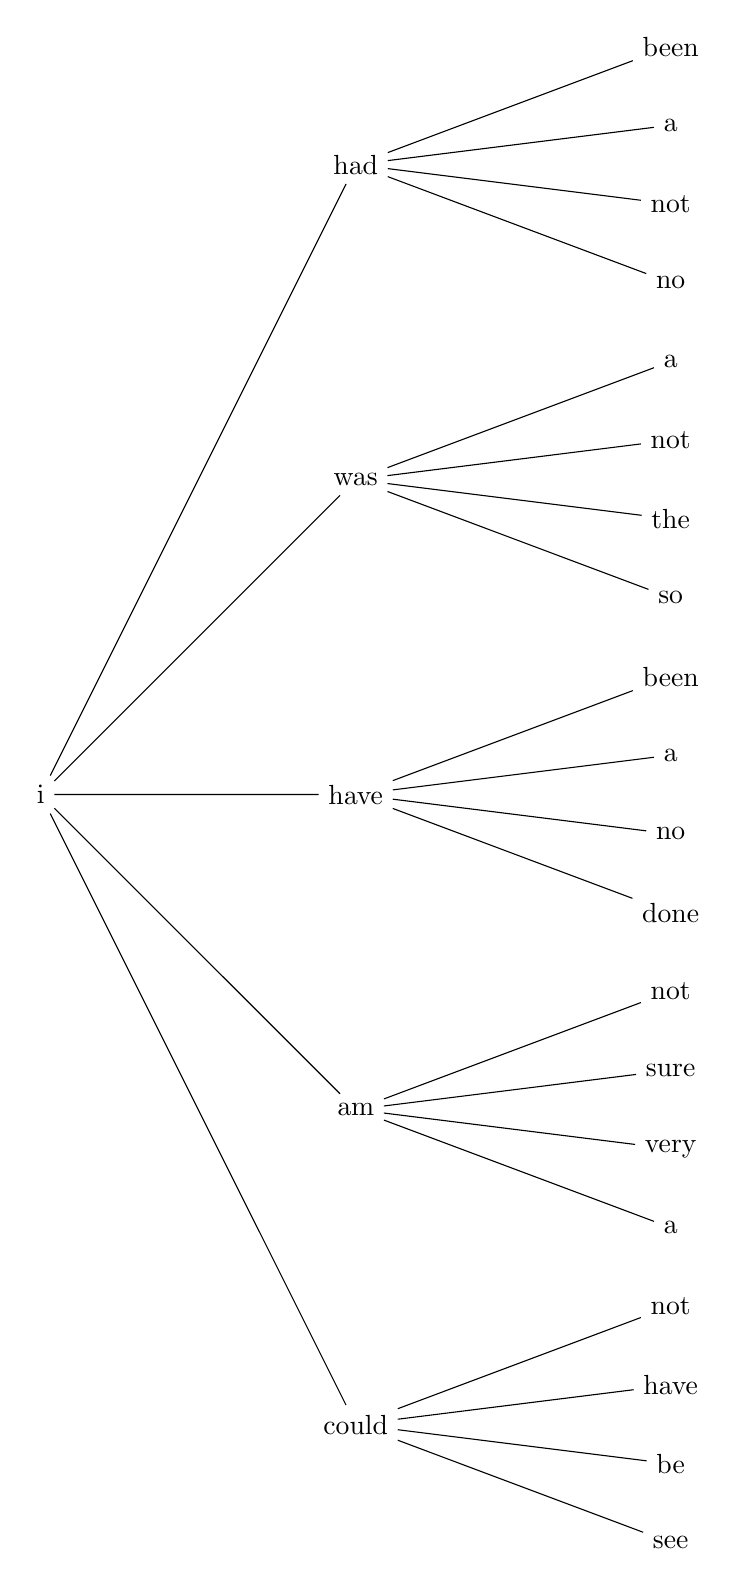
\begin{tikzpicture}[grow'=right,
  level distance=4cm,
  level 1/.style={sibling distance=4cm},
  level 2/.style={sibling distance=1cm}]
  \node {i}
    child {node {had}
      child {node {been}}
      child {node {a}}
      child {node {not}}
      child {node {no}}
    }
    child {node {was}
      child {node {a}}
      child {node {not}}
      child {node {the}}
      child {node {so}}
    }
    child {node {have}
      child {node {been}}
      child {node {a}}
      child {node {no}}
      child {node {done}}
    }
    child {node {am}
      child {node {not}}
      child {node {sure}}
      child {node {very}}
      child {node {a}}
    }
    child {node {could}
      child {node {not}}
      child {node {have}}
      child {node {be}}
      child {node {see}}
	};
\end{tikzpicture}
\caption{Results with seed 'i'}
\end{figure}

Below are three sentences generated using the same algorithm, but only picking the most probable next word. The seed word is the first word in the sentence: 
\begin{lstlisting}
The old gentleman. 
It was a little em'ly. 
I had been a little em'ly.
\end{lstlisting}

\subsection{Creating Sentences Using a Random Walk}
With the Graphframe and Markov chain class set up, all that needs to be done is repeatedly call $nextState$ on the Graphframe to create the sentences. 

\begin{lstlisting}[language=python]
sentences = ""
markovChain = MarkovChain(graphFrame, startWord)
    while numSentences > 0:
        currentState = markovChain.getState()
        if currentState in string.punctuation:
            numSentences-=1
        sentences+= markovChain.getState() + " "
        markovChain.nextState()
\end{lstlisting}

This will continue generating words and sentences until it is told to stop by hitting the amount of sentences specified. But, because of the properties of Markov chains, it will start out being heavily dependent on the start word. However, if the chain is let to run long enough, its dependence on the start word deteriorates due to it approaching the limiting state of the chain.
\linebreak
\linebreak
Sentences generated with MCMC methods: 
\begin{itemize}
\item a solemn consideration, he wished otherwise, was away or four years and it a fan at present?
\item what do you leave me, it every blade of course of waste
\item i had ordered to me the stable-door, picking himself down again they are as to his was hanging
\end{itemize}

\subsection{Drawbacks}
The sentences above show some of the drawbacks using this method. While the model does predict sentences that follow Dicken's structure, notice that the sentences do not necessarily make sense. This is due to the memoryless property of Markov chains that prevents the model from making decisions based off past words or states. This leads to sentences that use similar words and tone as the author, but very rarely make sense or have any meaningful context. Also, due to memorylessness, sentences will not transition into one another. Once the chain is at the punctuation state, it has no obligation to follow any sort of flow of the previous sentence as the chain only cares about the current state. 

\section{Other Uses For MCMCM}
In general, Markov chain Monte Carlo methods can be used to create a generative model for any dataset. One example of this is modeling stock market data. If Markov chain Monte Carlo methods are given stock market data, it will try and predict future states based off of what has happened in the past. Again, due to memorylessness of Markov chains, it will only try and predict based off of the current state's price point. While not perfect at modeling complex data that depends on previous states, like stock markets, the fact that the chain relies on historical data as a basis should provide some level of accuracy. 
Some other interesting uses could include breaking simple encryption algorithms like a Caesar cipher or replacing each letter with a new symbol. This is done by the exact same process that is used to generate the most common word, except each vertex is a letter and not a word. Then, instead of just predicting the most common letter, it uses a random walk MCMC algorithm to create the correct map from the code to the original language.\cite{Diaconis:4} Similarly, Markov chain Monte Carlo methods can be used for author detection. If there is a book with an unknown author and it is believed to be written by, for example, Charles Dickens, Markov chain Monte Carlo methods can be used to determine if the unknown book is probably written by Charles Dickens. By compiling the books known to be written by Charles Dickens into a Markov chain and the unknown book into another, the two chains can be compared through statistical analysis. If the analysis passes a set metric (as determined appropriately by the specific scenario), then it can be reasonably predicted that the unknown book was written by, in this example, Charles Dickens.

\section{Alternate Methods}
An alternate method that could be added to making the chain is applying Laplace smoothing to the edge weights. Laplace smoothing typically makes any values tend more towards a mean and not extreme values. For example, if there are two edges from a vertex and one value is very high and the other is very low, Laplace smoothing will increase the low value and decrease the high value. Mathematically, 
\begin{equation}
P_{new} = \dfrac{\alpha + \lambda}{d + \lambda V}
\end{equation}
where $P_{new}$ is the new probability, $\alpha$ is the amount of times the word appears in the text, $d$ is the total amount of words, $V$ is the amount of unique words, and $\lambda$ is a scalar.\cite{Hockenmaier:6}
This can be of use because if the data is very rigid it might not have the proper distribution that is desired; the rigidness of the edge values could only be an artifact of the data picked. So the smoothing would then try and fix this by having the values tend toward the average.

Also, the accuracy of the generative model could be greatly increased by taking into account more previous states. In the models generated above, future words were generated based on only one word(the current word). If the future word was dependent on the current word and the word that proceeded the current word, the sentences generated would make more contextual sense. This could be implemented by instead of each vertex consisting of only one word, there also was a vertex that has a bigram.
\section{Conclusion}

The implementation of Markov chains to model any joint-probability based data using Apache Spark and GraphFrames allows for a highly scalable basis for creating a generative model. Specifically, it can be used to generate sentences that have the same stylistic frequencies and traits of the texts passed into the model. This model can then be used to cross-reference styles to determine the probable source of a text or just generate stock sentences in the same style as the inputs.

\section{Acknowledgements}
Special thanks go to Quinn Jarrell, Bhuvan Venkatesh, Professor Robert J. Brunner, and the rest of the CS199 staff for providing the knowledge needed to complete this project. We would also like to thank the National Center for Supercomputing Applications for providing us with the Nebula cluster. 


\begin{thebibliography}{1}
\bibitem{Laurie:1}
Grinstead, C. M., Snell, J. L. (2006). Introduction to probability. Providence: American Mathematical Society. Retrieved April 25, 2017, from https://www.dartmouth.edu/\~chance/teaching\_aids/books\_articles/
probability\_book/Chapter11.pdf

\bibitem{Hunter:2}
Hunter, T., \& Bradley, J. (2016). Graphframes package. Retrieved April 25, 2017, from https://graphframes.github.io/api/python/graphframes.html

\bibitem{Sigman:3}
Sigman, Karl. "Markov Chains II: Recurrence And Limiting (Stationary) Distributions". http://www.columbia.edu/. N.p., 2009. Web. 25 Apr. 2017.

\bibitem{Diaconis:4}
Diaconis, P. (2008, August 22). The Markov Chain Monte Carlo Revolution. Retrieved April 25, 2017, from http://statweb.stanford.edu/~cgates/PERSI/papers/MCMCRev.pdf

\bibitem{Ng:5}
Ng, A. Y., \& Jordan, M. I. (2002, September 22). On Discriminative vs. Generative classifiers: A comparison of logistic regression and naive Bayes. Retrieved April 25, 2017, from https://ai.stanford.edu/~ang/papers/nips01-discriminativegenerative.pdf

\bibitem{Hockenmaier:6}
Hockenmaier, Julia. "Lecture 3: Smoothing". Fall 2012. Lecture.
\end{thebibliography}


\end{document}